\section{Deployment and Operation Galactic Radio Explorer} \label{sec:GReXOtheWork}

The Galactic Radio Explorer (GReX) is an all sky radio monitor developed specifically to detect exceptionally bright fast transients like FRBs \citep{shila_grex_2025,stare2SGR}. This project succeeds the similarly designed STARE2 which successfully detected FRB 200428 in 2020 \citep{stare2SGR}. The GReX instrument itself is a low cost instrument, the feed itself is a modified "cake-pan" which was chosen specifically for its wide beam which is about 70 deg at 1400 MHz and with a frequency range of 1280-1530~MHz. GReX is also equipped with the same LNAs as the deep synoptic array which has a noise temperature of about 7~K \citep{weinreb_low_2021, ravi_dsa-110_2023}. The antenna is then directly attached to a frontend module (FEM) which is below the feed (see \cref{fig:GReXOverview}) which handles down conversion, filtering, gain control and monitoring diagnostics. 

\begin{figure}[h]
    \centering
    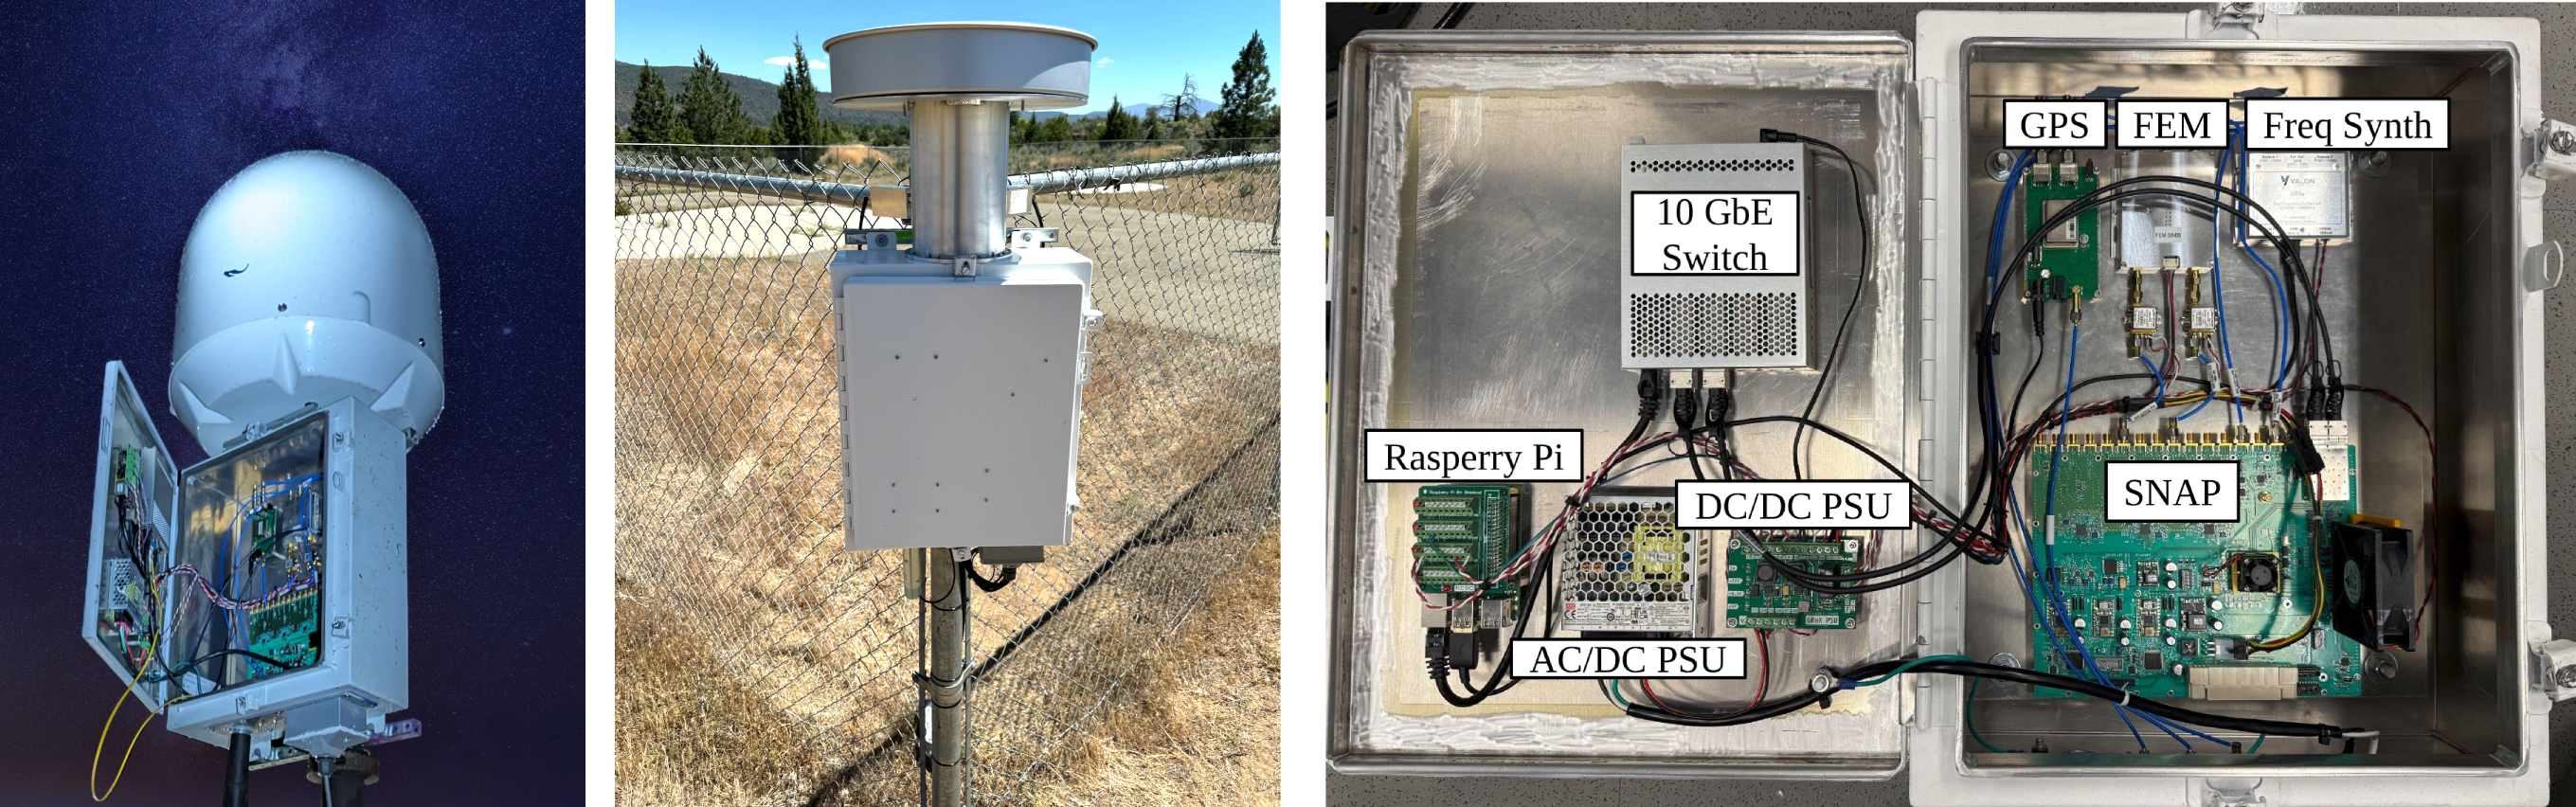
\includegraphics[width=\linewidth]{chapter8/figs/grex/GReX_overview.png}
    \caption{Pictures of GReX units based at Birr \textit{(left)} and HCRO \textit{(middle)}, the Birr unit has a weatherproof radome covering the cake pan feed which can be seen on the HCRO unit. The \textit{right} is a labelled diagram of the contents inside a GReX box which contains the signal chain.}
    \label{fig:GReXOverview}
\end{figure}

Along with the FEM there is a GPS, frequency synthesizer (oscillator), 10~GbE switch and the SNAP board. The SNAP board acts as the digitizer and FPGA platform for GReX. It is equipped with three ADCs and a Kintex-7 FPGA. The FPGA channelizes each polarization into 2048 frequency bins and then streams the 8-bit complex voltages over the Ethernet switch with a throughput of 8 Gb/s to a compute server. Timing comes from a GPS with a 10~MHz reference which timestamps the samples at the packet level, this allows for $32.768~ \upmu \rm s$ time resolution. For more details on the unit design see \cite{connor_galactic_2021} and \cite{shila_grex_2025}. 

On the software side, GReX captures packets where RFI cleaning, de-dispersion and \textsc{Heimdall} used to find candidates. If a candidate is found a filterbank is dumped to disk on the connected server and candidate plots are sent into the GReX slack. 

The purpose of GReX is to be a cheap and open source self constrained instrument that can be deployed with minimal access to infrastructure. At present there are four GReX units operating at OVRO, Cornell, Harvard, HCRO and Birr with two more planned to be deployed at Parkes in New South Wales, Australia and Gauribidanur, India. The following sections detail work carried out in commissioning the HCRO and Birr units along with carrying out a self generated RFI analysis conducted with both units along with some of the key science results of operation. 

\begin{figure}[h]
    \centering
    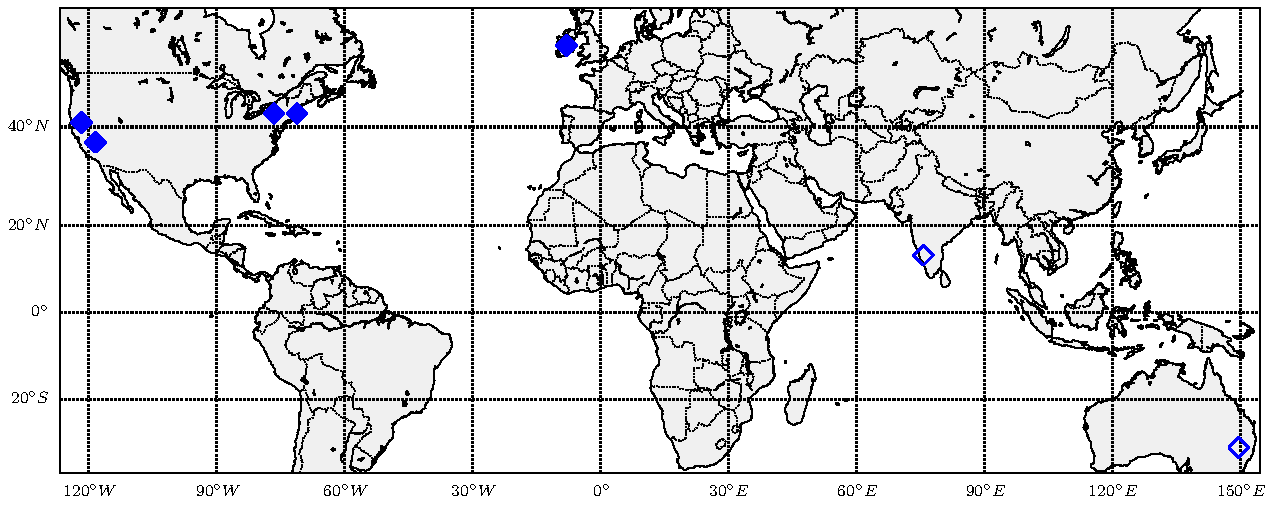
\includegraphics[width=\linewidth]{chapter8/figs/grex/GReX_Ground_Deployments_Map.pdf}
    \caption{Mercator map with deployed and on-sky GReX stations ($\blacklozenge$) along with stations at various stages of deployment ($\lozenge$).}
    \label{fig:ground-deployments}
\end{figure}

\subsection{Hat Creek Radio Observatory}

The GReX deployment at HCRO was completed in June 2024. Before installation, the box was first tested in a screened room using a spectrum analyzer connected to an omnidirectional antenna and external amplifier. Measurements were conducted with the GReX unit turned off for baseline measurements and then powered on with the box both open and closed with RF absorbers placed inside the enclosure. Steel wool was added to the fiber cable opening to enhance shielding.
These measurements (discussed in \cref{sec:self_rfi}) show that the self-generated RFI is stronger than expected, and necessitated installation at a more remote location on-site to avoid interference with other experiments.

\subsection{Rosse Observatory}
The deployment of the GReX unit in Ireland was completed in December 2024 at the radio observatory of Trinity College Dublin. The Rosse Observatory is situated in Birr, in the relatively low population density Irish Midlands. The site already hosts the Irish LOw Frequency Array (LOFAR) station~\citep{lofar,ilofar} and other smaller experiments.
As the GReX deployment was in close proximity to the LOFAR station, any unintended emission from the GReX unit in the LOFAR band was measured in the lab, prior to deployment. Due to the harsher weather conditions in Ireland, the GReX unit underwent further waterproofing with extra sealant on the box where all components are housed (see \cref{fig:GReXOverview}). The most notable modification is the use of a radome housing, as it is radio transparent and often used on marine vessels to protect equipment from harsh outdoor elements.

\begin{figure}[h]
    \centering
    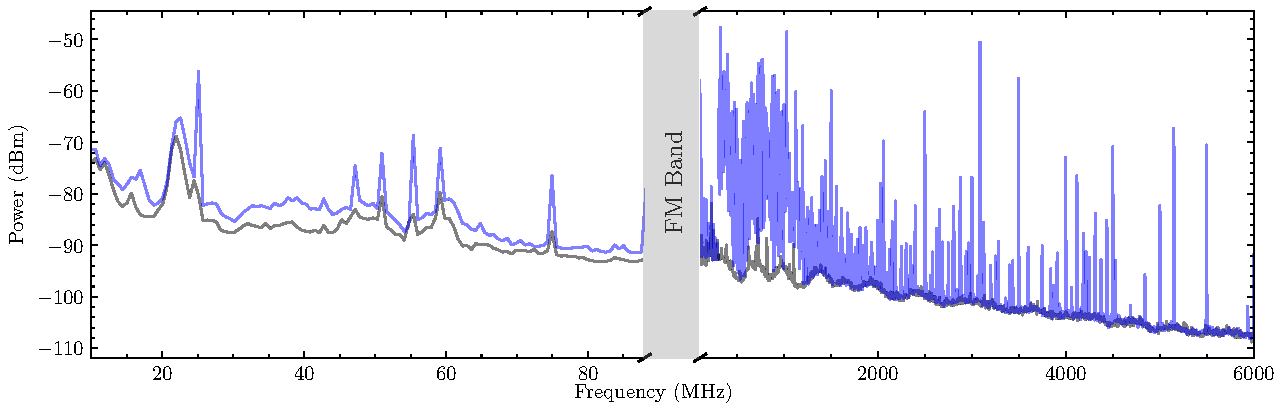
\includegraphics[width=\linewidth]{chapter8/figs/grex/GReX_Ground_Deployments_withFoV.pdf}
    \caption{Measured power spectrum from $10-6000\,\text{MHz}$ of a closed GReX box.
    The blue trace shows the spectrum when the unit is powered on, while the gray trace represents the baseline measurement.
    The frequency range of $10-300\,\text{MHz}$ was measured at Birr in a lab and $300-6000\,\text{MHz}$ was measured at HCRO in a screened room.}
    \label{fig:GReXRFISpectrum}
\end{figure}

\subsection{Self-Generated RFI} \label{sec:self_rfi}

As GReX is intended to be hosted at radio observatories as well as universities, tests of the self-generated RFI are critical to maintain spectrum purity at sensitive sites.
Lab tests of the box's emission were performed at HCRO and Birr, but not at OVRO due to lack of resources. Additionally, Stokes I data were taken using I-LOFAR at Birr while GReX was operational. The lab tests of the closed box's emission are shown in \cref{fig:GReXRFISpectrum}.
The results from the tests at HCRO in the $300-6000\,\text{MHz}$ band indicate that GReX in its current form is not yet suitable for installation close to sensitive telescopes observing in this band. We believe the RFI retrofitting of the commercial enclosure used to house the electronics is primarily at fault. Further experiments with other RFI gaskets and conductive tape show a marked improvement in radiated power, but not totally acceptable for sensitive sites, especially at L-band. However, Stokes I data from I-LOFAR (shown in \cref{fig:GReXIE613-sst-test}) show no appreciable contamination. Additionally, the various ongoing experiments at OVRO such as the DSA-110 and LWA have also not noticed any increase in local RFI.

While some mitigations have substantially improved the unit's radiated power, the box remains a moderate RFI source. The self-generated RFI has not proven to be an issue for the FRB detection pipeline, nor has it interfered with experiments at operational radio observatories. However, the emission remains an open issue and prevents installation at some sites. Further work is needed to identify problematic components and improve shielding.


\begin{figure}[h]
    \centering
    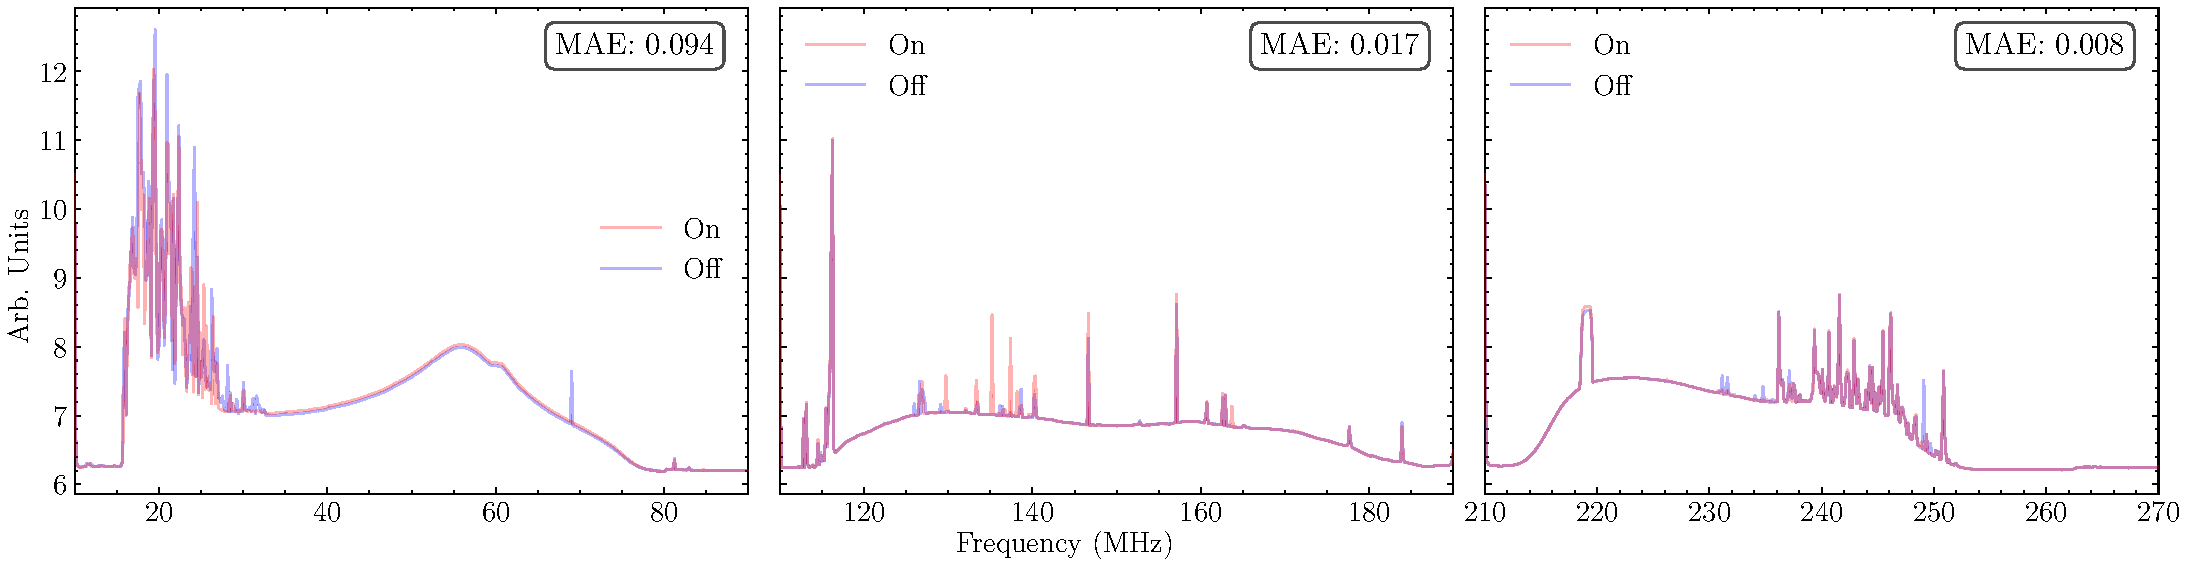
\includegraphics[width=\linewidth]{chapter8/figs/grex/sst_test.pdf}
    \caption{15-minute Stokes I spectra measured using I-LOFAR with the GReX unit powered on and off, covering all observing modes from $10-270\,\text{MHz}$. The mean absolute error (MAE) was calculated for each measurement, comparing the powered-on spectrum to the baseline (powered-off) measurement.}
    \label{fig:GReXIE613-sst-test}
\end{figure}

\subsection{Technosignature Searches}

GReX units can be used to carry out technosignature surveys.
GReX's large field of view enables the constraining of upper limits on the prevalence of intelligent life in the local galaxy.
Presently, two technosignature pipelines can be deployed. 
A high-spectral-resolution technosignature detection pipeline can be deployed to search for drifting narrowband technosignatures.
In the case of GReX, coincidence rejection from two or more units can be used to mitigate non-terrestrial narrowband signals \citep{johnson_simultaneous_2023}.
Additionally, artificially dispersed signals can be searched for, as described in \cite{gajjar_searching_2022}, by deploying \textsc{SPANDAK}\footnote{\url{https://github.com/gajjarv/PulsarSearch/}} on GReX.
The minimum power of a transmitter that can be detected is given in terms of effective isotropic radiated power (EIRP), for a narrowband signal, this is expressed as

\begin{equation}
    \text{EIRP}_\text{min,narrow}(f, l, b) = \sigma \cdot 4\pi d_\star^2  \frac{2 k_b T_{\text{sys}}(l, b)}{A_e(f)}  \frac{1}{\sqrt{n_p  t_\text{obs}  \delta\nu}}.
\end{equation}

Here, $\sigma$ is the required signal-to-noise ratio (SNR), $\delta\nu$ is the bandwidth of the received signal, $t_{\text{obs}}$ is the observing integration time, $A_e(f)$ effective area of the telescope as function of frequency, $T_{sys}(l,b)$ system temperature as a function of sky position, $n_p$ is the number of polarizations, and $d_\star$ is the distance between the transmitter and receiver, i.e., the distance to the star.
A value of 1~Hz is assumed for $\delta\nu_t$. For narrowband signals considered in Doppler searches. Similarly, an artificially dispersed signal can be expressed as
\begin{equation}
    \text{EIRP}_\text{min,disp}(f, l, b) = \sigma \cdot 4\pi d_\star^2  \dfrac{2 k_b T_{\text{sys}}(l, b)}{A_e(f)}  \dfrac{1}{\sqrt{n_p ~\delta \nu ~ \tau}}.
\end{equation}

However, in this case $\tau$ represents the pulse duration of the dispersed burst where 1~ms is assumed.
A technosignature emanated from Alpha Centauri (1.34~pc) would require $1.2\times10^{12}\,\text{W/Hz}$ and $4.9\times10^{12}\,\text{W/Hz}$ for a dispersed burst and a narrowband signal at an SNR of 10.
Here the maximum effective area of GReX is used along with a $T_{sys}$ of $50\,\text{K}$.
The wide FoV of GReX places it as a useful tool in characterization of potential technosignatures enabling meaningful constraints in the observing band.  

\subsection{Upper Limit of Bright FRBs}

The main science case for GReX is dectecting Galactic FRBs \citep{stare2SGR}. At the time of writing GReX hasn't detected any Galactic FRBs. Thus, an upper limit can be placed on prevalence of FRBs in the Galaxy. Modelling the burst arrivals as a Poisson process with a rate $\lambda$ over an effective observing time, $\tau$. Where the Poission probablity distribution is, 

\begin{equation}
    p(k|\lambda,\tau) = \frac{(\lambda\tau)^ke^{-\lambda\tau}}{k!}\,,
\end{equation}

To estimate the event rate $\lambda$ when $k=1$, the above equation is rearranging for $p(k|\lambda,\tau)$ and solved using Bayes' theorem assuming a flat prior on $\lambda$ where $p(\lambda)\propto 1$ via


\begin{align}
        p(\lambda|k=1,\tau_1) = & \frac{p(k=1|\lambda,\tau_1)p(\lambda)}{p(k=1|\tau_1)}\\
        =&\frac{\lambda\tau_1e^{-\lambda\tau_1}}{\int_{0}^{\infty}d\lambda \lambda\tau_1e^{-\lambda\tau_1}}\\
        =& \tau_1^2\lambda e^{-\lambda\tau_1}.
    \label{eq:k1_p}
\end{align}

This results in a  posterior that is a Gamma distribution with shape parameter, $k+1$ and rate parameter $\tau_1$. For a single detected event $(k=1)$, this becomes a $\Gamma(2,\tau_1)$ distribution.
Here $\tau_1$ is taken to be the effecting observing time GReX. Only the GReX unit is used for an upper limit as at the time of publication of \citet{shila_grex_2025} it had been observing consistently since May 2024 when it took over from its predecessor STARE2 \citep{stare2SGR}. This amounts to 6.3 yrs observing with both STARE and GReX at OVRO, with 12\% instantaneous sky sensitivity and assuming the unit was  operational 75\% of the time the effective observing time is $0.567$ sky y, where one sky year corresponds to one year of continuous monitoring of the entire sky. \Cref{fig:posteriors_FRBs_Grex} shows the posterior distributions for event rate, $\lambda$ under the assumed observing exposure. Including the additional observing time accumulated after the detection of FRB 200428, during which no further events were detected, all-sky event rate for FRBs above $\sim 50~\rm kJy$ as 8.37 $\text{sky}^{-1}\text{yr}^{-1}$ \citep[see appendix A for telescope calibration,][]{shila_grex_2025}. The GReX units require little intervention and continuously observe to date, more up-to-date limits will be presented in the future work. 

\begin{figure}[h]
    \centering
    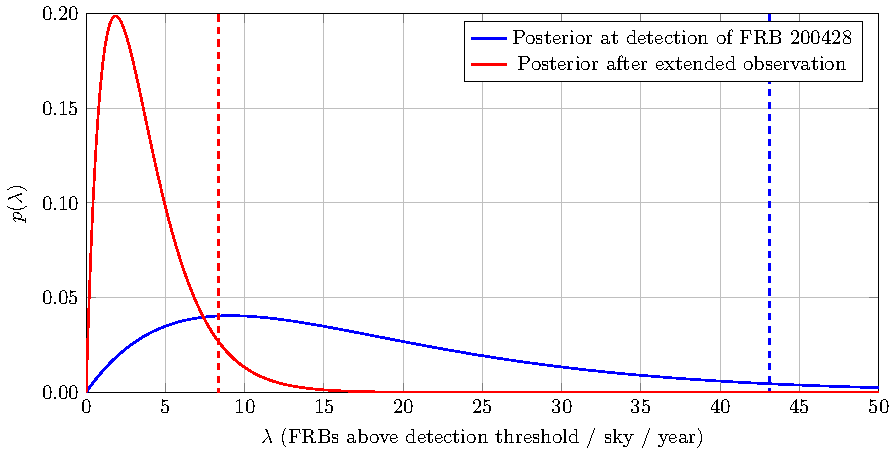
\includegraphics[width=\linewidth]{chapter8/figs/grex/rate_pdfs.pdf}
    \caption{Posterior distribution of FRB event rate $\lambda$ with associated dashed 95\% confidence upper limits \citep{shila_grex_2025}}
    \label{fig:posteriors_FRBs_Grex}
\end{figure}